\documentclass{beamer}
%\usepackage[spanish,activeacute]{babel}
\usetheme{metropolis}
\usepackage[utf8]{inputenc}
\usepackage{listings}
\usepackage{amsmath,amsfonts,amssymb}
\usepackage{color}
\usepackage{tikz}
\usetikzlibrary{positioning}
\usepackage{array}
%\usepackage{graphicx}
\usepackage{adjustbox}
\usepackage{booktabs}
\usetikzlibrary{shapes,arrows}
%\usepackage{multicol}
\usepackage{hhline}
\usepackage{pgf}
\usepackage{algorithm} 
\usepackage{algorithmic}
\renewcommand{\algorithmicrequire}{\textbf{Input:}}
\renewcommand{\algorithmicensure}{\textbf{Output:}}
\def\R{{\mathbb R }}
\def\N{{\mathbb N }}




\definecolor{BlueTOL}{HTML}{222255}
\definecolor{BrownTOL}{HTML}{f43d00}%666633}
\definecolor{GreenTOL}{HTML}{225522}
\setbeamercolor{normal text}{fg=BlueTOL,bg=white}
\setbeamercolor{alerted text}{fg=BrownTOL}
\setbeamercolor{example text}{fg=GreenTOL}

\metroset{block=fill}

\setbeamercolor{block title alerted}{use=alerted text,
    fg=alerted text.fg,
    bg=alerted text.bg!80!alerted text.fg}
\setbeamercolor{block body alerted}{use={block title alerted, alerted text},
    fg=normal text.fg,
    bg=block title alerted.bg!50!alerted text.bg}
\setbeamercolor{block title example}{use=example text,
    fg=example text.fg,
    bg=example text.bg!80!example text.fg}
\setbeamercolor{block body example}{use={block title example, example text},
    fg=example text.fg,
    bg=block title example.bg!50!example text.bg}


%\author[Paola Arce]{Paola Arce \\ Departamento de Inform\'atica, UTFSM \\ Thesis advisor: Luis Salinas}
%\date{December 15, 2017}
%\title[Thesis defense]{Online learning methods for financial time series forecasting}
%\subtitle{PhD Thesis Defense}
%
%\titlegraphic{
%    \tikz[overlay,remember picture]
%        \node[at=(current page.south east), anchor=south east] {
%            
\includegraphics[height=1.5cm]{img/DIT}
%        };
%}

\author[Paola Arce]{Paola Arce \\ Thesis advisor: Luis Salinas}
\date{December 11, 2017}
\title[Thesis defense]{Fast and adaptive cointegration based model for forecasting financial time series}
\subtitle{Seminario Inform\'atica CCTVal}



\begin{document}

\begin{frame}[plain]
\titlepage
\begin{tikzpicture}[overlay, remember picture]
\node[above right=0.4cm and 1.2cm of current page.south west] {
\includegraphics[width=2.5cm]{img/UTFSM}};
%\node[above =0.5cm of current page.south] {
\includegraphics[width=2cm]{img/DIT}};
\node[above left=0.5cm and .8cm of current page.south east] {
\includegraphics[width=5cm]{img/logo-di}};
\end{tikzpicture}

\end{frame}
%\usebackgroundtemplate{ } 

\begin{frame}
\frametitle{Outline}
\begin{itemize}
\item Motivation: High Frequency trading
\item Cointegration and the VECM model
\item Challenges and Hypothesis
\item Contributions
\item Experiments
\item Conclusions
\item Future work
\end{itemize}
\end{frame}

\section{Motivation}

\begin{frame}
\frametitle{HFT: High Frequency Trading}
High frequency trading has motivated computer-driven strategies capable of processing large amount of data in short periods of time.
\begin{figure}
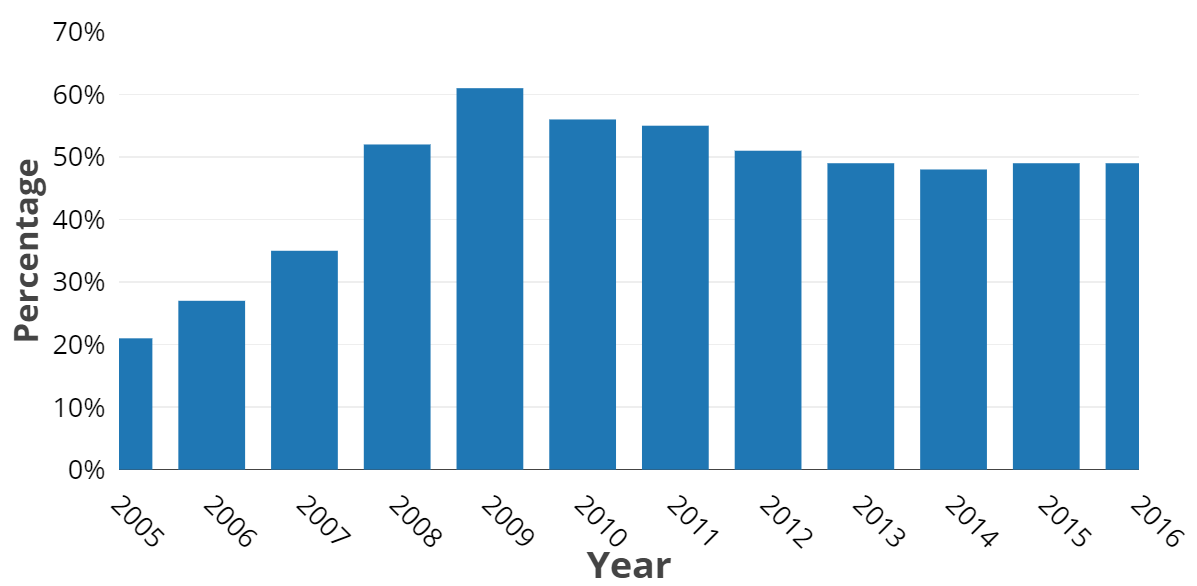
\includegraphics[width=0.7\paperwidth]{img/HFTmarket}
\caption{Percentage of HFT trades of total US Equity Trading. Source: TABB group}
\end{figure}
\end{frame}


\begin{frame}
\frametitle{HFT Revenue}
However, the revenues have fallen dramatically mainly because of more regulation, increasing cost of HFT infrastructure and more competitive algorithms.
\begin{figure}
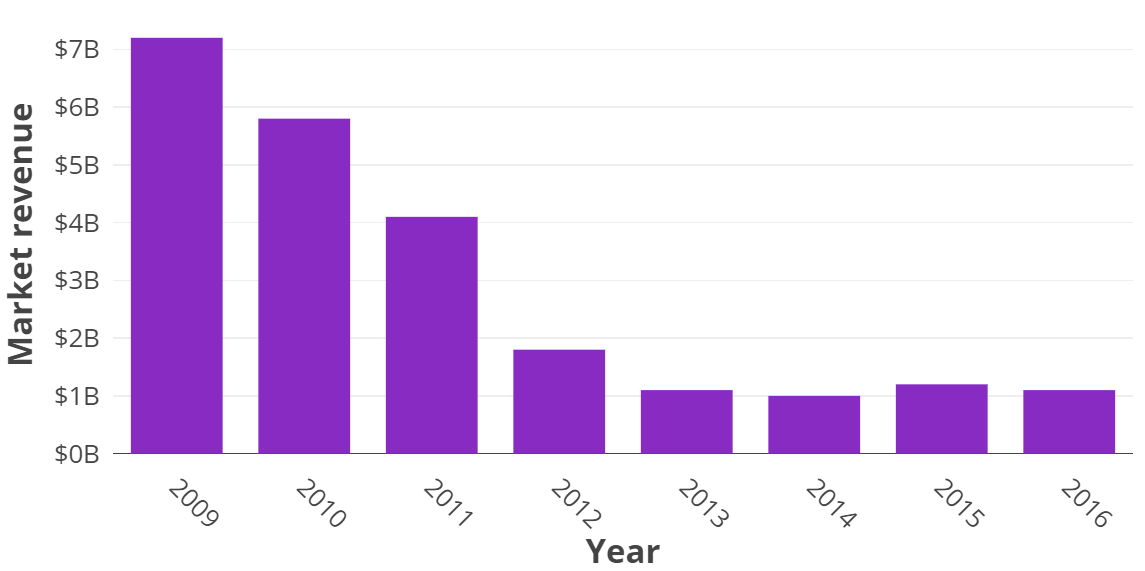
\includegraphics[width=0.7\paperwidth]{img/HFTmarket2}
\caption{Revenue in the US. Source: TABB group}
\end{figure}
\end{frame}


\begin{frame}
\frametitle{High Frequency data}
High frequency time series are commonly:
\begin{columns}
\begin{column}{0.5\textwidth}
\begin{itemize}
\item Non-stationary
\item Irregularly spaced over time.
%\item Heterogeneity
\item Heteroscedastic
\item Potentially cointegrated
\end{itemize}
\end{column}
\begin{column}{0.5\textwidth}
\begin{figure}
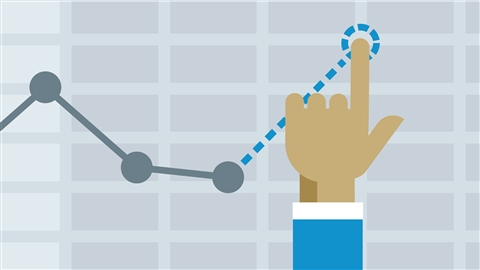
\includegraphics[width=0.35\paperwidth]{img/forecast}
\end{figure}
\end{column}
\end{columns}
\vspace{5mm}
This imply that classical statistical models can't be used. Therefore, financial time series forecasting is still a challenge.
\end{frame}

\begin{frame}
\frametitle{Stationarity}
\begin{block}{Strong definition}
A {\color{red}strictly stationary time series} $y_t \in \mathbb{R}$, $\forall t \in \mathbb{Z}$ is one for which the probabilistic behaviour of every collection of values $\{y_{t_1},y_{t_2},\dots,y_{t_L}\}$ is identical
to that of the time shifted set, more precisely:
\begin{equation*}
{\color{blue}
P\{y_{t_1} \leq
c_1,..,y_{t_L} \leq c_L\} = P\{y_{t_1+h} \leq c_1,..,y_{t_L+h} \leq c_L\}\enspace }
\end{equation*}
\noindent $\forall L \in \mathbb{N}, \forall h \in \mathbb{Z}$ where $c_1,\dots,c_L$ are constants.
\end{block}
\end{frame}

\begin{frame}
\frametitle{Stationarity}
\begin{block}{Weak definition}

A weakly stationary time series is a process which mean, variance and auto covariance do not change over time:
\small
{\color{blue}
 \begin{eqnarray*} E(y_t) &=& \mu  \quad
\forall t \in \mathbb{N} \\ E(y^2_t) &=& \sigma^2  \quad \forall t \in
\mathbb{N} \\ \lambda(s,t)&=&\lambda(s+h,t+h) \quad \forall s,t \in \mathbb{N},
\forall h \in \mathbb{Z} \end{eqnarray*}}
\end{block}
\noindent with $\lambda(s,t) = E[(y_s-\mu)(y_t - \mu)]$ 
\end{frame}

\begin{frame}
\frametitle{Stationarity: consequences}
One of the consequences of stationary processes is how they recover from a shock. A shock represents an unexpected change in a variable in a particular period of time. For stationary time series, shocks to the system will gradually die away. 
\begin{figure}
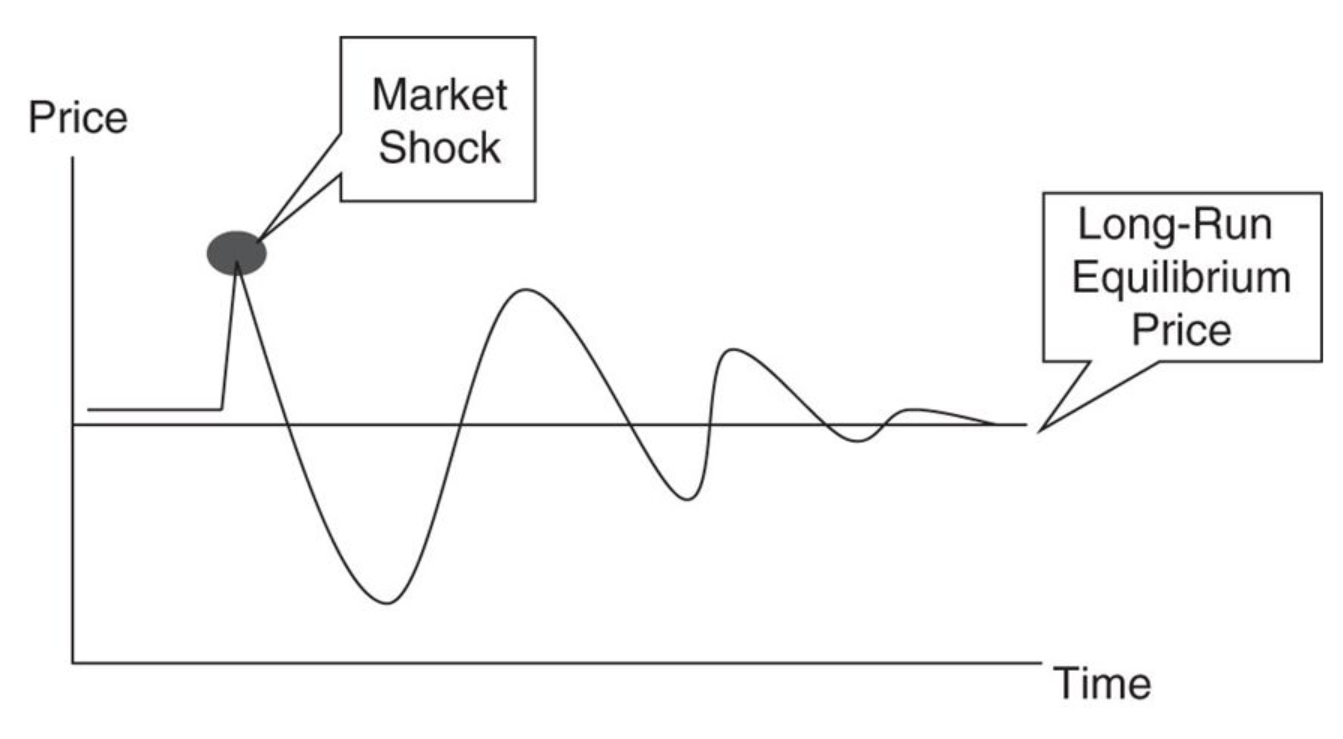
\includegraphics[width=0.6\paperwidth]{img/shock}
\end{figure}
\end{frame}


\begin{frame}
\frametitle{Non-stationary processes}
There are different types of non-stationary time series models often found in economics. Unit root process is one of them commonly used to model prices:
\begin{block}{Unit root process}
{\color{red}Unit root or I(1)} processes are also called stochastic trend if they have the following form:
{\color{blue}
\[
y_t = \mu + y_{t-1} + \epsilon_t
\]}
\noindent where $\epsilon_t$ is a stationary process. When $\mu = 0 $ the process is called {\bf pure random walk} and when $\mu \neq 0$  the process is called {\bf random walk with drift}.
\end{block}
\end{frame}


\begin{frame}
\frametitle{Integration }
\begin{block}{Integration of order $d$}
A time series $\mathbf{y}$ is said to be I(d), or integrated of order $d$, if after
differentiating the variable $d$ times, we get an stationary process, more precisely:
\[
{\color{blue}
(1-L)^d \mathbf{y} \sim \text{I(0)}} \, ,
\]
\noindent where I(0) is a stationary time series and $L$ is the lag operator:
\[
(1-L)\mathbf{y} = \Delta \mathbf{y}=\mathbf{y}_t  -\mathbf{y}_{t-1} \quad \forall t
\]
\end{block}
\end{frame}

\begin{frame}
\frametitle{Irregularly spaced over time}
\begin{figure}
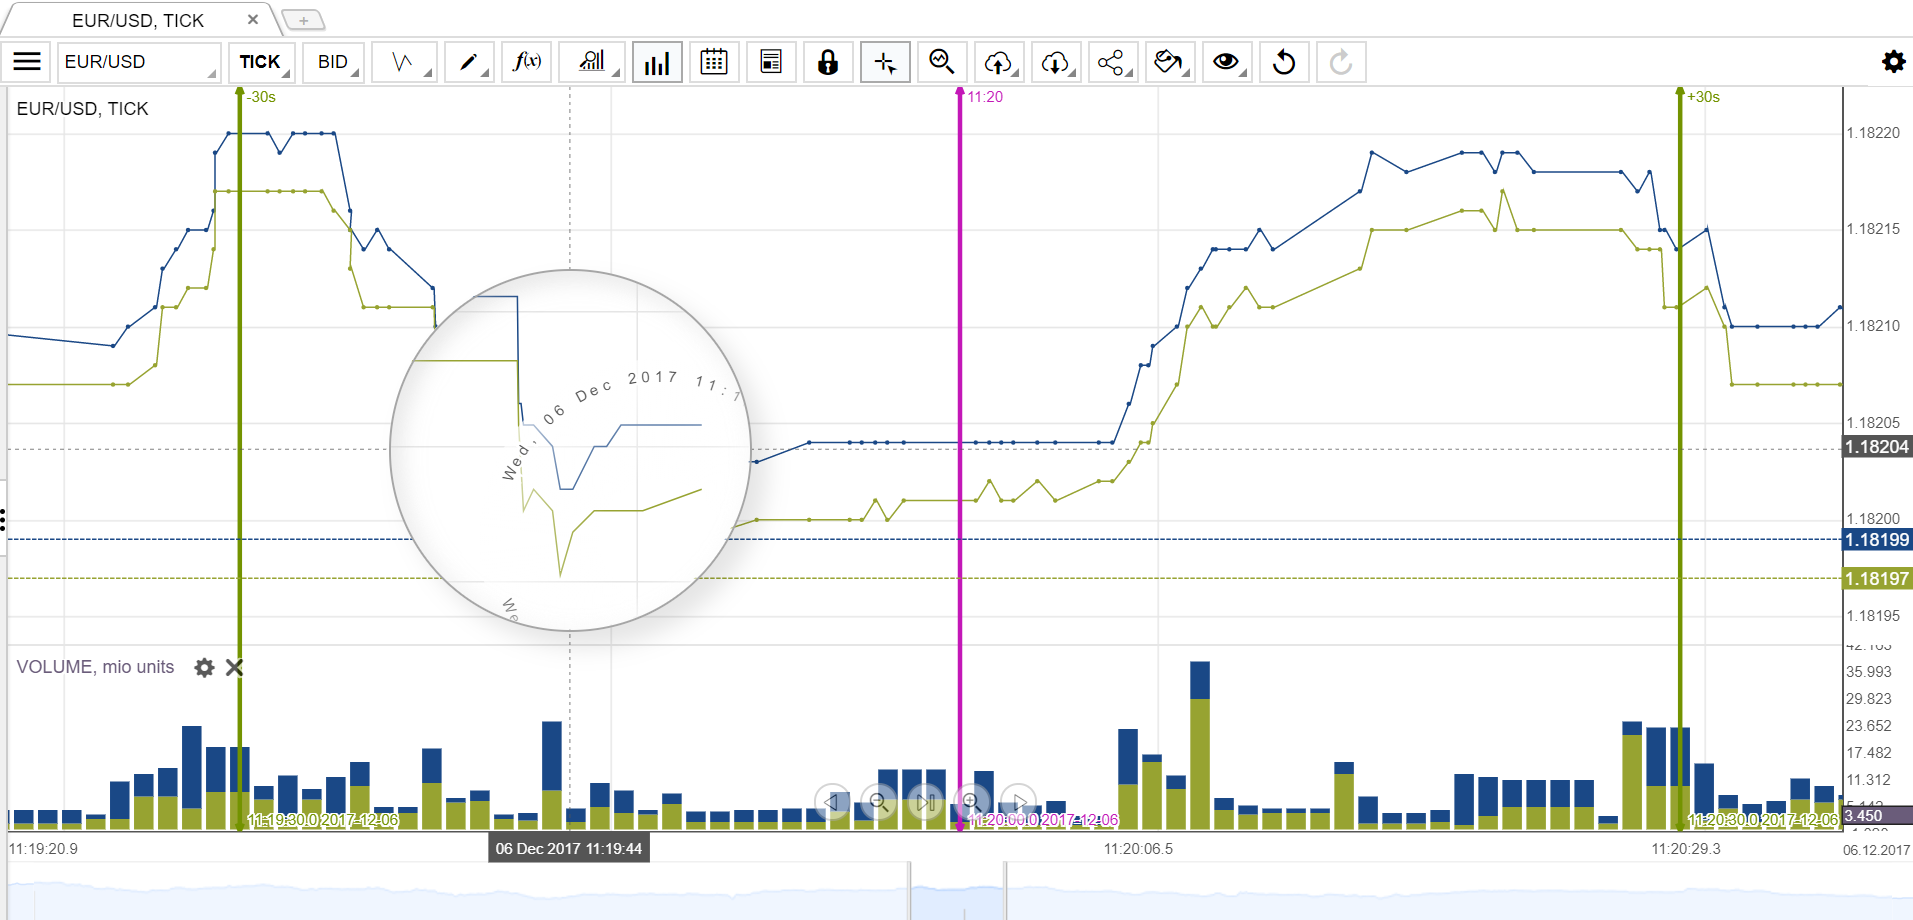
\includegraphics[width=0.8\paperwidth]{img/hft-ticks-zoom.png}
\end{figure}
\end{frame}

\begin{frame}
\frametitle{Heteroscedastic}
Conditional heteroskedasticity identifies non-constant volatility.
Volatility gives a measure of uncertainty about future returns. Many factors affect volatility such as: historical prices, trends, monetary policies and news.
\begin{figure}
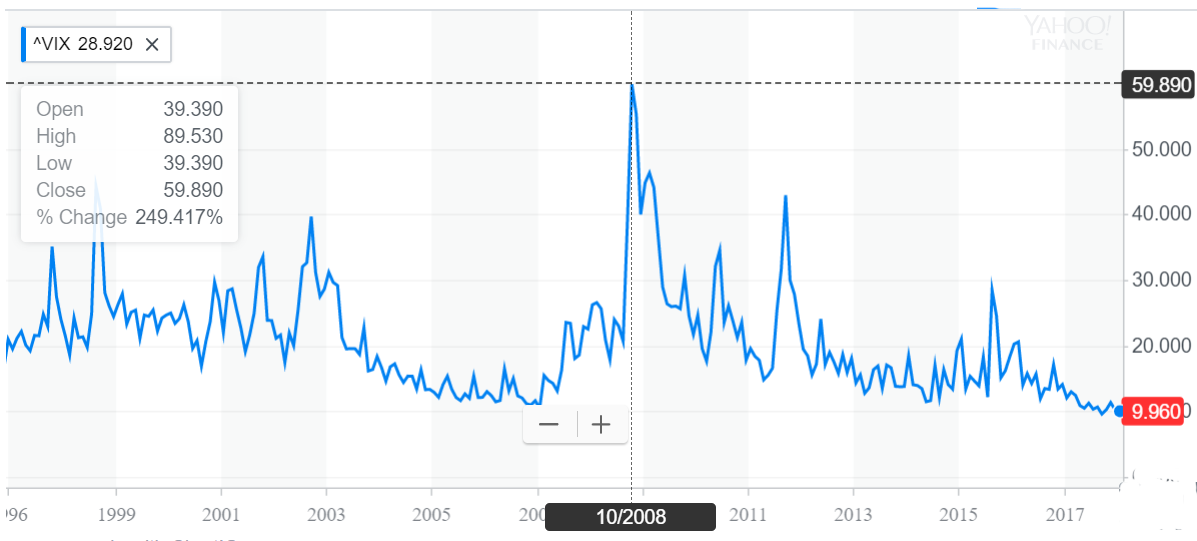
\includegraphics[width=0.8\paperwidth]{img/vix}
\end{figure}
\end{frame}

\section{Cointegration and the VECM model}
\begin{frame}
\frametitle{Cointegration}
\begin{figure}
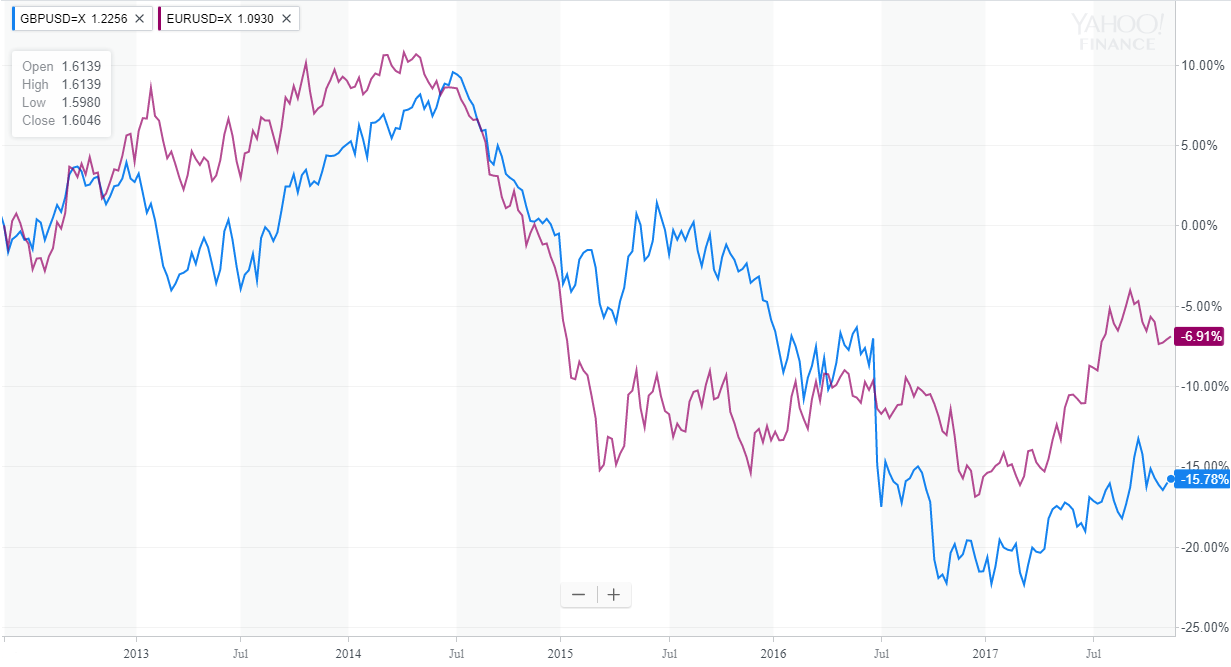
\includegraphics[width=0.8\paperwidth]{img/motivation}
\end{figure}
\end{frame}

\begin{frame}
\frametitle{Cointegration definition}

\begin{block}{Cointegration}
The relationship between non-stationary time series can be modelled if a {\bf stationary linear combination} is shown to exist.
When this happens it is said they have a {\bf long-run
equilibrium} relationship and the variables are {\color{red} cointegrated}.
\end{block}


\end{frame}

\begin{frame}
\frametitle{Cointegration: formal definition}
\begin{block}{Cointegration definition}
Let {\color{blue}$\mathbf{y} = \{\mathbf{y}^1, \dots, \mathbf{y}^l\}$} be a set of $l$
time series of order I(1) which are said to be cointegrated if a vector
${\color{blue}\boldsymbol\beta=[\beta(1),\dots,\beta(l)]^\top} \in \mathbb{R}^l$  exists such that the
time series,

\begin{equation*}
 \mathbf{Z}_t:= \boldsymbol \beta^\top \mathbf{y} = \beta(1) \mathbf{y}^1 + \dots + \beta(l) \mathbf{y}^l \sim
 \text{I(0)}\, .
\end{equation*}
\end{block}
%In other words, a set of I(1) variables is said to be cointegrated if
%a linear combination of them exists which is I(0).

\end{frame}


\tikzstyle{every picture}+=[remember picture]
\everymath{\displaystyle}
\begin{frame}
\frametitle{The Vector Error correction}
\tikzstyle{na} = [baseline=-.5ex]

The Vector Error correction model (VECM) is used to model cointegrated time series:

{\Large
\begin{equation*}
 \Delta \mathbf{y}_t = \underbrace{
        \tikz[baseline]{
            \node[fill=red!20,ellipse,anchor=base] (t1)
            {$ \Omega\mathbf{y}_{t-1}$};
        }}_\text{Error correction term} +
        \underbrace{
        \tikz[baseline]{
            \node[fill=blue!20,anchor=base] (t2)
            {$\sum_{i=1}^{p-1} \phi_i^* \Delta \mathbf{y}_{t-i} $};
        }}_\text{Autorregresive term} +
        \underbrace{
        \tikz[baseline]{
            \node[fill=green!20,anchor=base] (t3)
            {$c$};
        }}_\text{Intercept}
        +
        \underbrace{
        \tikz[baseline]{
            \node[fill=yellow!20,anchor=base] (t3)
            {$\mathbf{\epsilon}_t $};
        }}_\text{i.i.d}
\end{equation*}
}
\noindent where $p$ is the number of lags and $\boldsymbol \Omega = \boldsymbol \alpha \boldsymbol \beta^\top$. The columns of $\boldsymbol\beta$ contains the cointegration vectors and the rows of $\boldsymbol\alpha$ correspond with the adjusted vectors.
\end{frame}


\begin{frame}
\frametitle{$\boldsymbol \Omega$ matrix properties}
The matrix $\boldsymbol \Omega$ has the following properties:
\begin{itemize}
\item If ${\color{blue}\boldsymbol \Omega = 0}$ there is no cointegration
\item If ${\color{blue}rank(\boldsymbol\Omega)=l}$ i.e full rank, then the time series are not
I(1) but stationary
\item If ${\color{blue}rank(\boldsymbol\Omega)=r,\quad 0 < r < l}$ then, there is cointegration.
%where $\boldsymbol\alpha$ and $\boldsymbol\beta$ are $(l \times r)$
%matrices and $rank(\boldsymbol\alpha)=rank(\boldsymbol\beta)=r$.
\end{itemize}
\end{frame}


\begin{frame}
\frametitle{VECM limitations}

\begin{alertblock}{VECM limitations}
The Vector Error correction model is used to model cointegrated time series but only with {\bf batch data and rarely used with high frequency data} mainly due to {\bf computational limitations}:
\begin{itemize}
\item Calculation of the cointegration vectors $\boldsymbol \beta$ is obtained by the Johansen procedure which is of order $O(n^3)$.
%whereas $\alpha$ has to be determined as a variable in the VECM.
\item VECM parameters are obtained using the ordinary least squares ({\bf OLS}) method.
\end{itemize}
\end{alertblock}
\end{frame}


\section{Challenges and Hypothesis}
\begin{frame}
\frametitle{Challenge}
\begin{block}{Proposal}
To adapt VECM to be used with high frequency data, where the best parameters are updated when new data arrives.
\end{block}
\begin{exampleblock}{Hypothesis}
An algorithm based on cointegration and high performance computing will allow faster forecasting
algorithms for financial time series to be obtained while maintaining good accuracy levels.
\end{exampleblock}
\end{frame}

\section{Contributions}
\begin{frame}
\frametitle{First contribution: Adaptive VECM}
\hspace*{-9mm}
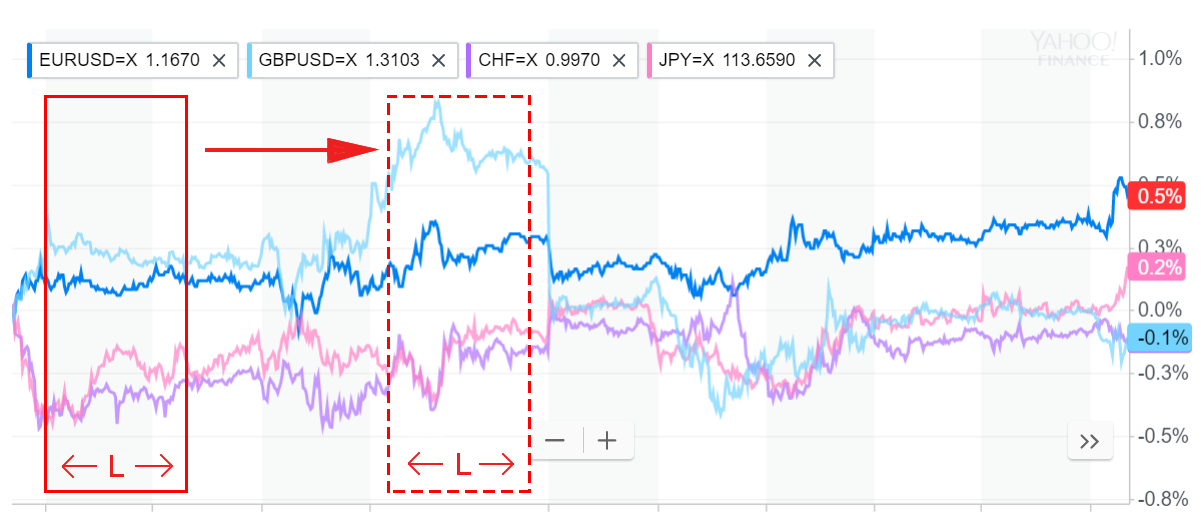
\includegraphics[width=1.15\textwidth]{img/slidingwindow}
\end{frame}

\begin{frame}
\frametitle{How to choose L?}
  \begin{figure}[!h]
  %\vspace{-0.8cm}
  \centering
   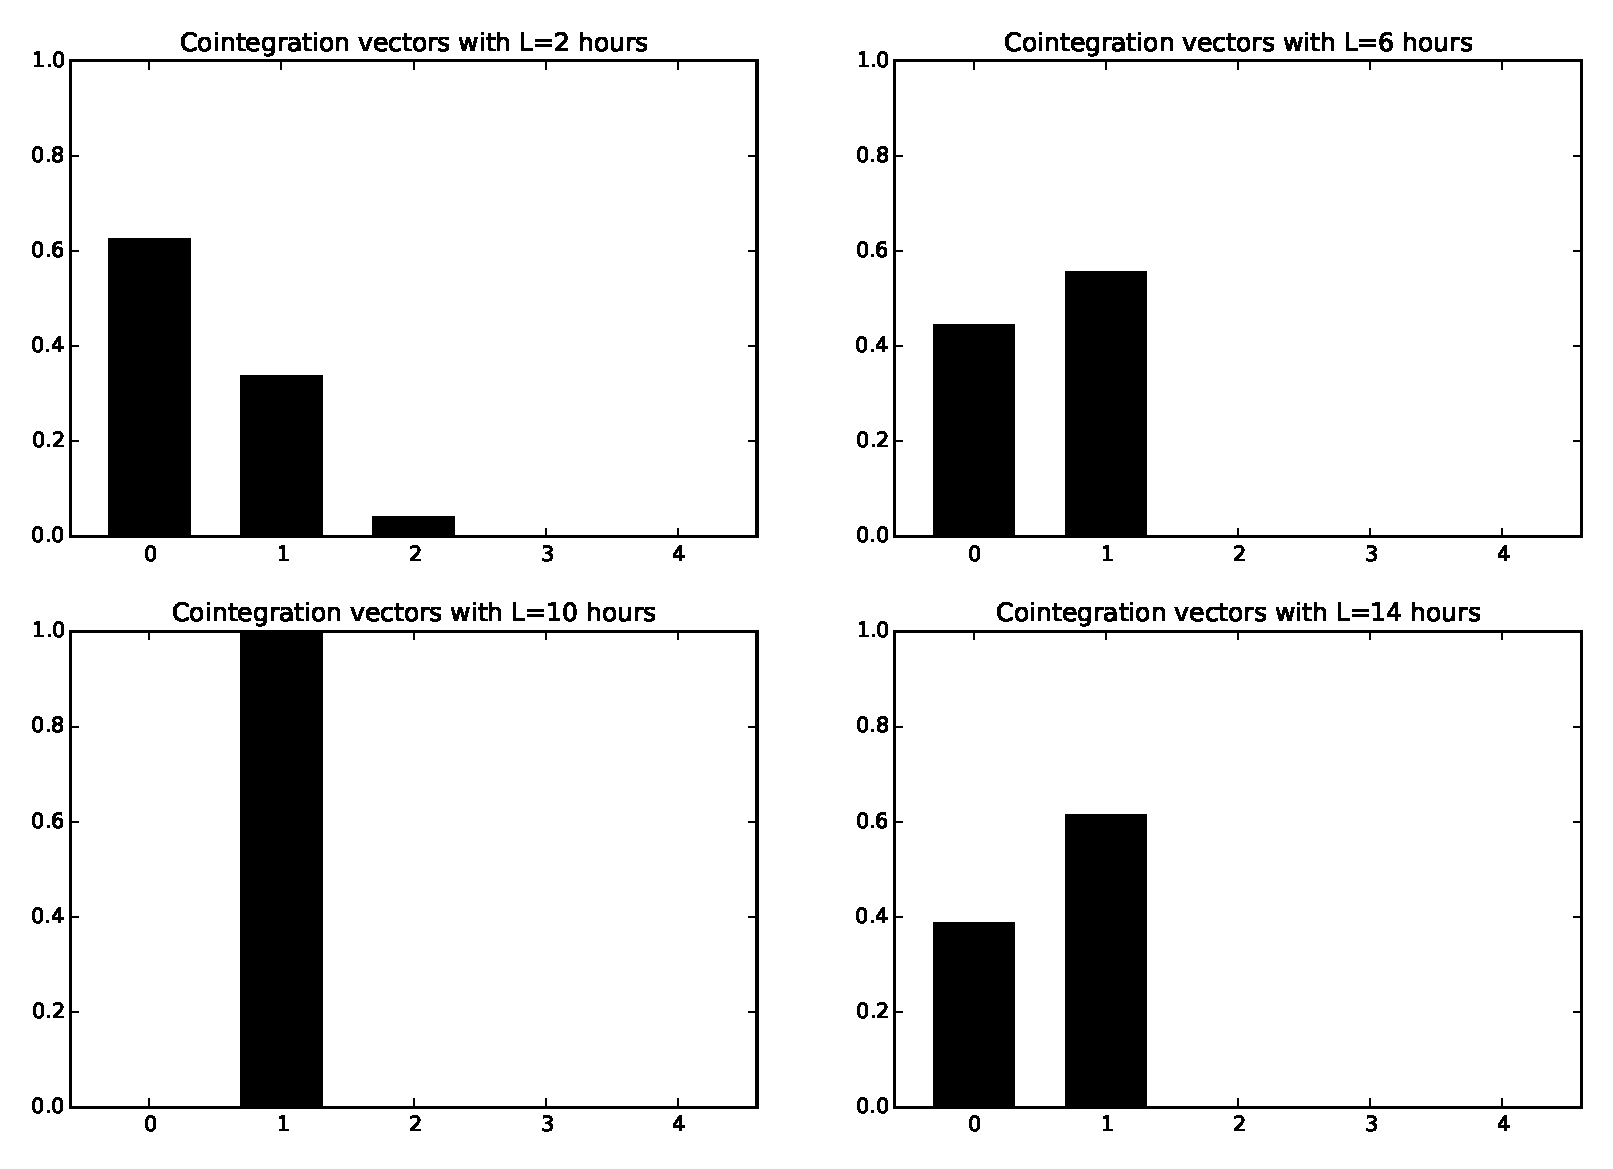
\includegraphics[width=0.85\textwidth]{img/51_Fig1}
  \caption[Distribution of the number of cointegration vectors using $p=1$ lags]{Distribution of the number of cointegration vectors using $p=1$ lags.}
  %Four possible values for windows size $L$ are shown (2, 6, 10 and 14) hours (1 hour = 360 data points).}
  \label{fig:hists}
\end{figure}
\end{frame}


\begin{frame}
\frametitle{Percentage of cointegration}
Since $r=0$ means no cointegration and $r=l=4$ reveals that no process is I(1) but stationary.
The interesting cases of cointegration are those where $r$ lies strictly
between $0$ and $l$, i.e. $0<r<l$.
\vspace{5mm}
\begin{block}{Percentage of cointegration (PC)}
{\color{blue}
\begin{equation*} \label{eq:pcoint}
PC = 
\frac{\#\{ it \mid \text{$it$ has $r$ c.v. with $0<r<l$}\}}
     {\#it}\times 100
\end{equation*}}
\end{block}
\end{frame}

\begin{frame}
\frametitle{Data}
\begin{columns}
\begin{column}{0.7\textwidth}
\begin{itemize}
\item This data was collected from {\bf Dukascopy}, a free
database which gives access to the {\bf Swiss Foreign Exchange marketplace}.
\item Tests were carried out using four foreign exchange rates all related to
USD: {\bf EURUSD, GBPUSD, USDCHF} and {\bf USDJPY}. 
\item The tests were done using 10-seconds frequency from ask prices
from the 11th to the 15th of August 2014. 
%\item Since one day corresponds to 8640 data points and we used 5 days of data, we have 43,200 data points in total.
\end{itemize}
\end{column}
\begin{column}{0.3\textwidth}
 \begin{figure}[!h]
    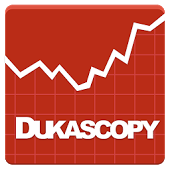
\includegraphics[width=\textwidth]{img/dukascopy}
 \end{figure}
\end{column}
\end{columns}
\end{frame}


\begin{frame}
\frametitle{PC vs MSE}
\begin{figure}[ht!]
  %\vspace{-0.8cm}
  \centering
  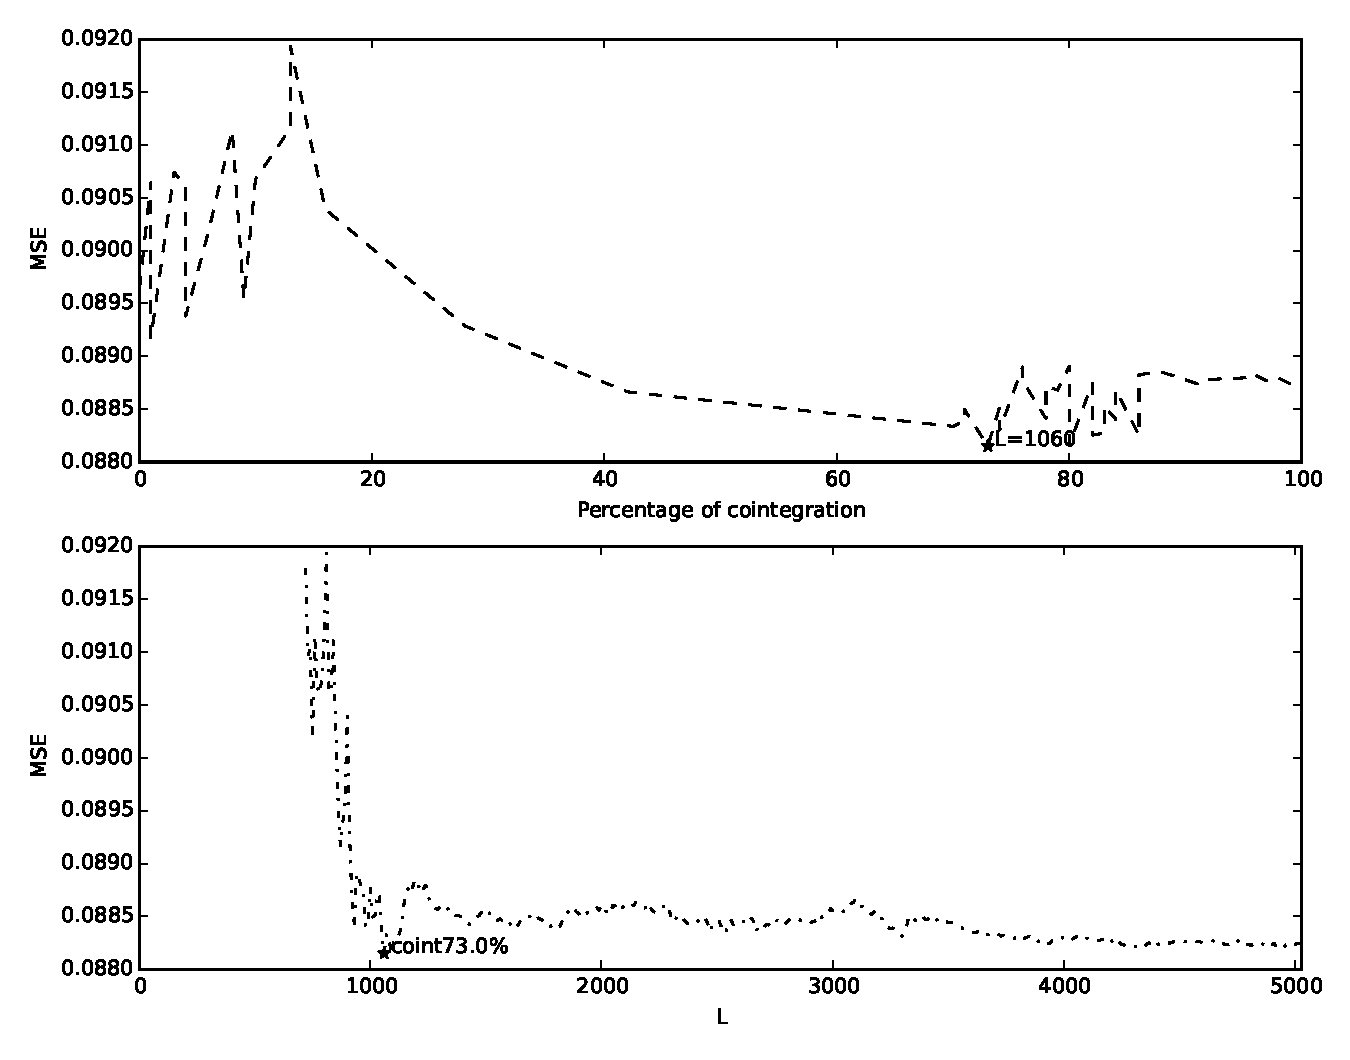
\includegraphics[width=0.7\textwidth]{img/51_Fig2}
  \caption{MSE versus the percentage of cointegration considering 1000
  iterations. }
  \label{fig:cointvsmse}
\end{figure}
\end{frame}

\begin{frame}
\frametitle{Adaptive VECM algorithm (AVECM)}
AVECM has the following features: 
\begin{enumerate}
\item Uses VECM only considering a sliding windows of size $L$ of data.
\item We proposed to choose $L$ and the number of lags $p$ in order to maximise the percentage of cointegration $PC$ in the near past. This process was done every time that new data was processed. 
\item To use a distributed environment to make this parameters search, since this is the most expensive routine.
\end{enumerate}
\end{frame}


\begin{frame}
\frametitle{AVECM Algorithm}
\small
\begin{algorithmic}[1]
\REQUIRE $\,$ \\
$\mathbf{y}$: matrix with $N$ input vectors and $l$ time series\\
$j$: Starting point of testing \\
$it$: Ending point of testing \\
$ps$: list of $p$ values \\
$Ls$: list of $L$ values ($L<N$) \\
$m$: Iterations to determine parameters ($m < N-L$)\\
\ENSURE  $\,$ \\
$\{ \hat{\mathbf{y}}[1],\dots,\hat{\mathbf{y}}[it]\}$: prediction vectors \\
\FOR { $i =j$ to $it$ }
   \STATE $\mathbf{Y} \gets \mathbf{y}[:,i-1]$
    \STATE $L,p \gets
    \texttt{get\_best\_params}(Ls,ps,m,\mathbf{Y})$
        \STATE $model = \text{VECM}(\mathbf{Y},L, p)$
        \STATE $\hat{\mathbf{y}}[i-j] = model.predict()$
\ENDFOR
\end{algorithmic}
\end{frame}




%%\begin{frame}
%%\frametitle{Evaluation methods}
%%\begin{block}{MSE}
%%Measures the distance between forecasts
%%and the true values and large deviations from the true value have a
%%large impact due to squaring forecast error.
%%{\color{blue}
%%\begin{equation}\label{eq:MSE}
%%\text{MSE} = 
%%\frac{\displaystyle \sum_{t=1}^{N} (\mathbf{y}_t-\hat{\mathbf{y}}_t)^2}{N}
%%\end{equation}}
%%\end{block}
%%\begin{block}{\bf $U$-statistic}
%%Unit free measure obtained as the ratio between the root MSE (RMSE) of a model and the RMSE of the naive random walk model. 
%%\end{block}
%%\end{frame}
%
%\section{Experiments}
%\subsection{Uno}
%
\begin{frame}
\frametitle{Unit root tests}
Augmented Dickey Fuller (ADF) test with lags $p=1,2,3,4,5$.
\begin{table}[ht]
\centering
\small
\begin{tabular}{llllll}
\toprule
{Variable} & {ADF(1)} & {ADF(2)} & {ADF(3)} & {ADF(4)} & {ADF(5)}\\ 
\midrule
EURUSD &  -0.052   & -0.054  & -0.054  & -0.054  & -0.054  \\
GBPUSD &  -0.744  & -0.784  & -0.805  & -0.837  & -0.846  \\
USDCHF &  -0.476   & -0.493  & -0.493  & -0.495  & -0.502  \\
USDJPY &  0.357   & 0.360  & 0.360  & 0.367  & 0.367  \\
$\Delta$ EURUSD & -128.4*  & -128.4*  & -96.85* & -89.12*   & -89.12*\\
$\Delta$ GBPUSD & -131.4*  & -112.7*  & -102.5* & -92.86*   & -88.29*\\
$\Delta$ USDCHF & -127.8*  & -127.8*  & -96.94* & -88.82*   & -80.79*\\
$\Delta$ USDJPY & -135.1*  & -135.1*  & -101.2* & -101.2*   & -101.2*\\
\bottomrule
\addlinespace[1ex]
\end{tabular}
\caption{Unit roots tests for EURUSD, GBPUSD, USDCHF and USDJPY at 10-second
frequency.}
\label{tab:adf}
\end{table}
\end{frame}

\begin{frame}
\frametitle{Performance accuracy}
\small
\begin{tabular}{ccccccc}
& \multicolumn{3}{l}{MSE} & &
\multicolumn{2}{c}{$U$-statistic} \\ 
\hhline{~---~--} \\
 & AVECM & ARIMA & p-value & &
AVECM & ARIMA \\ 

\hline
 EURUSD & 1.0702 e-09 & 1.1481 e-09 &  9.250 e-12 & & 0.6863 & 0.7108\\
 GBPUSD & 1.6630 e-09 & 1.7408 e-09 &  6.951 e-02 & & 0.6866 & 0.7025\\
 USDCHF & 5.8503 e-10 & 6.3545 e-10 &  2.899 e-14 & & 0.6803 & 0.7091\\
 USDJPY  & 6.3483 e-06 & 6.5194 e-06 &  6.853 e-05 & & 0.6964 & 0.7057
 \end{tabular}
 \end{frame}
%%For AVECM we considered different number of iterations (parameter $m$ in algorithm \ref{alg:AVECM}): 10, 50 and 100. We tried 12, 24 and 47 different pair of combinations for $L$ and $p$. Possible values for $L$ were in the interval $[100,4000]$ and $p$ can have values in between $[1,5]$. Best AVECM performance was compared against ARIMA and the random walk model.
%%Table~\ref{tab:stats} shows the out-of-sample performance measures: MSE and $U$-statistic for AVECM and ARIMA. In terms of both measures we found that AVECM is superior to ARIMA and the naive random walk model. We also included the p-value that proves that the difference in the MSE is significant at the 99\% significance level in three of the four currency rates and at 90\% in the case of GBPUSD. The $U$-statistic shows that AVECM and ARIMA are superior to the naive random walk model and that our proposal is also superior to ARIMA.
%
%
%
\begin{frame}
\frametitle{Parallel implementation}
The function that get optimal parameters $L$ and $p$ was implemented using MPI in Python. Tests ran in a cluster with 2 servers Xeon E5-2667 (2.90GHz) of 24 cores each (48 cores in total) and 24GB RAM.

Parameter settings:
\begin{itemize}
%\item Parameter $it=100$
\item The $L$ parameter was always chosen between 100 and 4000 and $p$ always took values between 1 and 5. 
\item Parameter $nparams$ represents the number of pairs ($L$,$p$) used to maximise the percentage of cointegration. 
\end{itemize}
\end{frame}
%
\begin{frame}
\frametitle{Execution times}
\begin{figure}[ht]
  \centering
  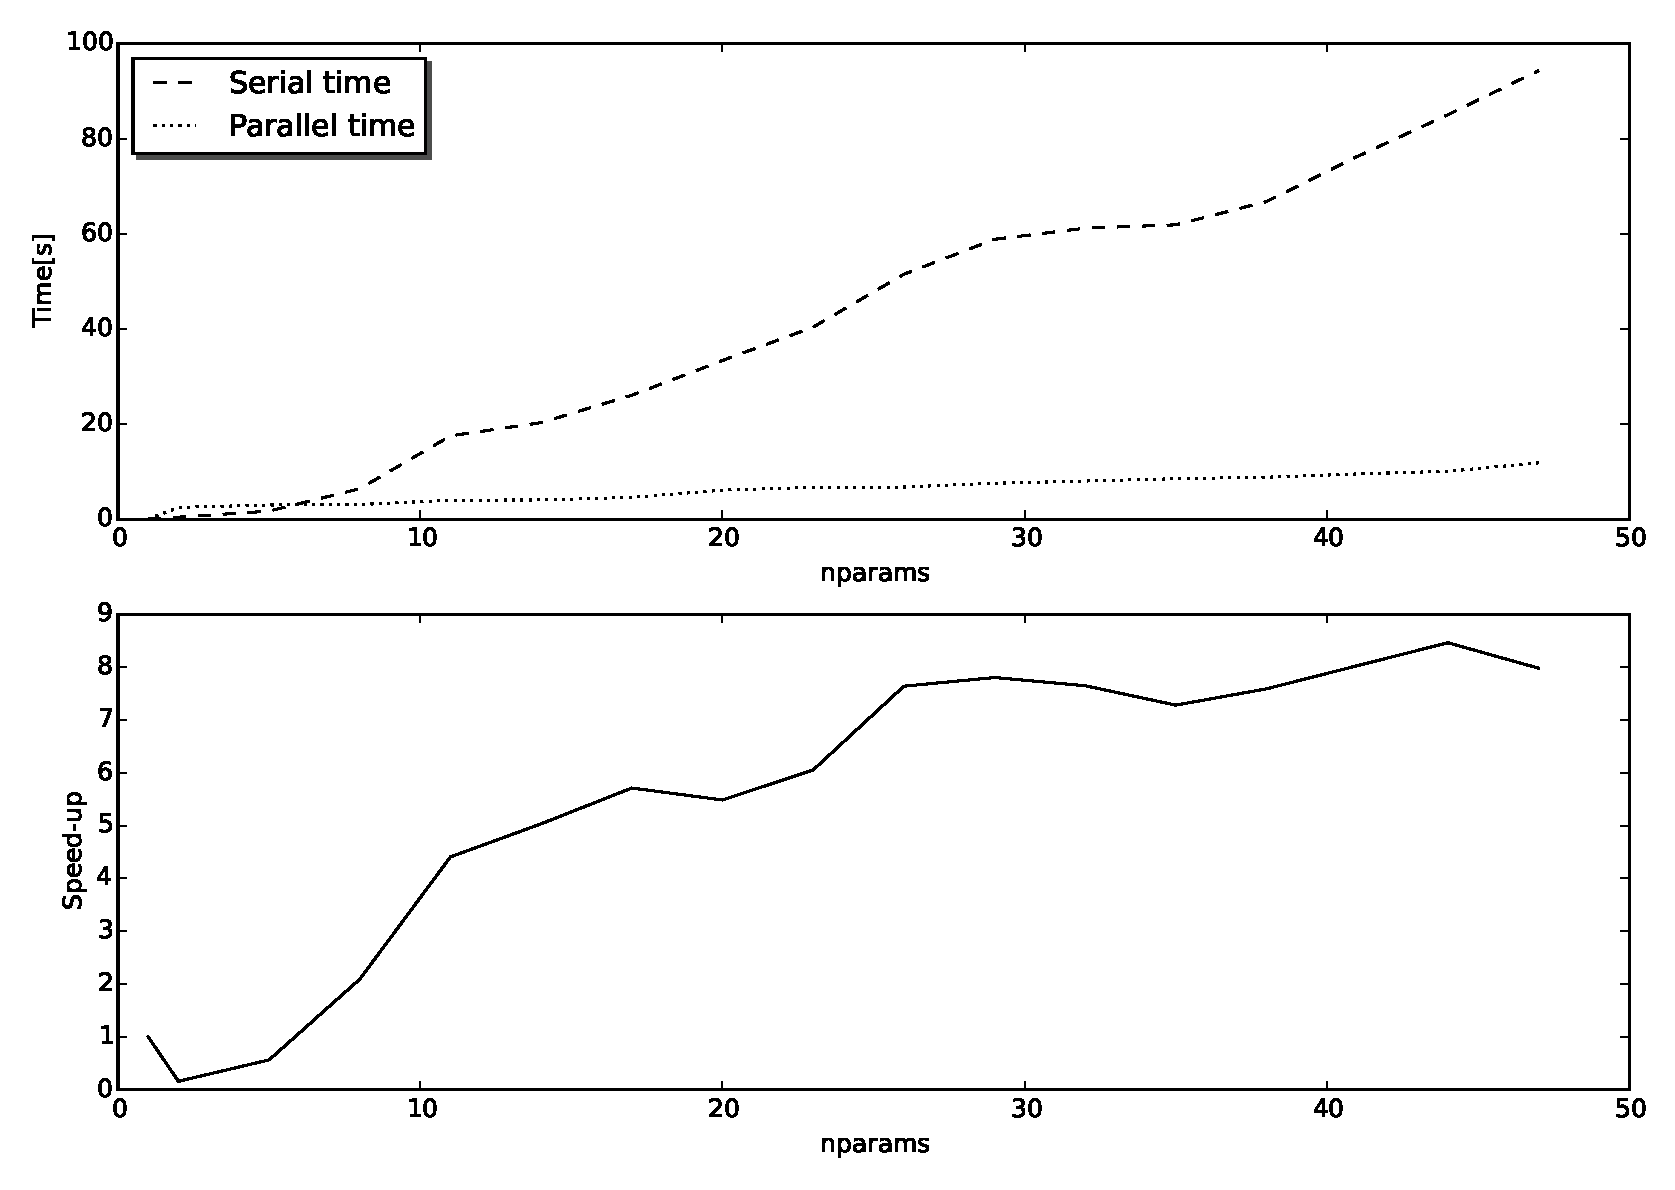
\includegraphics[width=0.9\textwidth]{img/51_Fig3}
  \caption[Computing time and Speed-up]{Computing time of sequential and parallel algorithm is shown in the
  upper figure. Speed-up is shown below.}
  \label{fig:extimes}
\end{figure}
\end{frame}

\begin{frame}
\frametitle{Conclusions}
\begin{itemize}
\item Cointegration relations change with time. We empirically showed that the Johansen method is sensitive to the number of lags but also to the amount of data considered.
%\item We found that out-of-sample forecast performance MSE is related to the {\em percentage of cointegration\/}.  
\item VECM improves performance measures by finding
parameters of $L$ and $p$ maximising the percentage of cointegration.
%\item Increasing the number of parameters will always lead to
%better performance measures.
\item The parallel implementation allowed the execution times to be reduced
more than 9 times and therefore a response time was obtain before 10
seconds. 
\end{itemize}
\end{frame}

\section{Second Contribution}

\begin{frame}
\frametitle{Second approach}
 Recently, online learning algorithms have been proposed to solve problems with large data sets because of their simplicity and their ability to update the model when new data is
available.
\begin{figure}
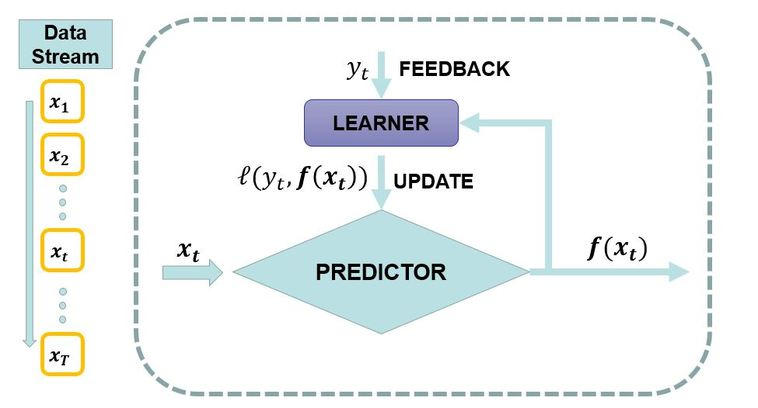
\includegraphics[width=0.6\paperwidth]{img/onlinelearning}
\end{figure} 
\end{frame}


\begin{frame}
\frametitle{Proposal: Online VECM algorithm (OVECM)}
\begin{itemize}
\item Considers only a sliding window of the $L$ most recent data. 
\item Since cointegration vectors represent long-run relationships they vary
little in time. OVECM obtains these vectors only when they need to be updated. 
\item This updating is done when MAPEs of the last $n$ inputs is above a certain
error given by a threshold 
\item OVECM also implements matrix optimisations in order to reduce execution time,
such as updating matrices with new data, removing old data and introducing new
cointegration vectors.
\end{itemize}
\end{frame}

\begin{frame}
\frametitle{Methodology}
OVECM were compared against VECM and ARIMA. VECM and ARIMA are called with a
sliding window of the most recent data, whereby the models are updated at every
time step. Therefore, we named them SLVECM and SLARIMA.
\end{frame}

\subsection{Parameters}
\begin{frame}
\frametitle{Parameters optimization}
VECM order and ARIMA parameters were selected using AIC.
\begin{table}[ht]
\label{tab:params}
\begin{center}
\begin{tabular}{|c|c|c|}
\hline
Windows size $L$ & VECM & ARIMA\\
 $L$ & order $(p)$ & order $(p,d,q)$ \\
\hline
100 & 2 & p=2,d=1,q=1\\
400 & 5 & p=1,d=1,q=1\\
700 & 3 &p=2,d=1,q=1\\
1000 &3 & p=2,d=1,q=1\\
\hline
\end{tabular}
\end{center}
\end{table}
\end{frame}

\begin{frame}
\frametitle{Execution times}
We ran 400 iterations of OVECM and SLVECM . SLARIMA was based on the ARIMA procedure
of the statsmodels library and therefore its execution time is excluded.
%because its is not comparable with OVECM and SLVECM. SLARIMA was created based
%on statsmodels library routine ARIMA.
\begin{center}
\adjustbox{max height=\dimexpr\textheight-5.5cm\relax,
           max width=\textwidth}{
\begin{tabular}{|l|c|c|c|c|c|}
\hline
& $L$ & order & e  & Time[s] \\
\hline
OVECM & 100 &p=2  & 0      & 2.492\\
OVECM & 100 &p=2  & 0.0026  & 1.606\\
SLVECM & 100 &p=2& -- & 2.100\\
\hline
OVECM & 400 & p=5  & 0      & 3.513\\
OVECM & 400 &p=5  & 0.0041  & 2.569\\
SLVECM & 400 & p=5 & -- & 3.222\\
\hline
OVECM & 700 &p=3  & 0      & 3.296\\
OVECM & 700 &p=3  & 0.0032  & 2.856\\
SLVECM & 700 &p=3 & -- & 3.581\\
\hline
OVECM & 1000 & p=3 & 0      & 4.387\\
OVECM & 1000 & p=3  & 0.0022  & 2.408\\
SLVECM & 1000 & p=3  & -- & 3.609\\
\hline
\end{tabular}
}\end{center}
\end{frame}

\begin{frame}
\frametitle{Performance accuracy}
\tiny
\begin{table}[H]
\caption{Model measures}
\label{tab:stats}
\begin{center}
\begin{tabular}{|l|l|c|c|c|c|c|c|c|}
\hline
\multicolumn{3}{|c|}{Model} & \multicolumn{3}{|c|}{In-sample} &
\multicolumn{3}{|c|}{Out-of-sample} \\ 
\hline
\hline
Method & $L$ & Parameters &  
MAPE & MAE& RMSE& 
MAPE & MAE& RMSE \\
\hline
 OVECM  &   100  &  P=2 e=0.0026 &  0.00263&  0.00085&  0.00114&  0.00309&  0.00094&  0.00131\\
 OVECM  &   400  &  P=5 e=0.0041&  0.00378&  0.00095&  0.00127&  0.00419&  0.00103&  0.00143\\
 OVECM  &   700  &  P=3 e=0.0032&  0.00323&  0.00099&  0.00130&  0.00322&  0.00097&  0.00132\\
 OVECM  &   1000 &  P=3 e=0.0022&  
 \textbf{0.00175}&  \textbf{0.00062}&  \textbf{0.00087} &  
 \textbf{0.00172}&  \textbf{0.00061}&  \textbf{0.00090}\\
\hline
 SLVECM  &   100 &  P=2 &  0.00262&  0.00085&  0.00113&  0.00310&  0.00095&  0.00132\\
 SLVECM  &   400 &  P=5 &  0.00375&  0.00095&  0.00126&  0.00419&  0.00103&  0.00143\\
 SLVECM  &   700 &  P=3 &  0.00324&  0.00099&  0.00130&  0.00322&  0.00098&  0.00132\\
 SLVECM  &   1000&  P=3 &  
 \textbf{0.00174}&  \textbf{0.00061}&  \textbf{0.00087}&  
 \textbf{0.00172}&  \textbf{0.00061}&  \textbf{0.00090}\\
\hline
SLARIMA & 100  &p=2 d=1 q=1 & 0.00285  &  0.00110  &  0.00308  &  0.00312  &0.00098  &  0.00144 \\
SLARIMA & 400  &p=1 d=1 q=1 & 0.00377  &  0.00101  &  0.00128  &  0.00418 & 0.00106 & 0.00145 \\
SLARIMA & 700  &p=2 d=1 q=1 & 0.00329  &  0.00102  &  0.00136  &  0.00324  & 0.00097  &  0.00133 \\
SLARIMA & 1000 &p=2 d=1 q=1 & \textbf{0.00281}  & \textbf{0.00074}  &  \textbf{0.00105}  &  \textbf{0.00177} & \textbf{0.00063}  &  \textbf{0.00092} \\
\hline
\end{tabular}
\end{center}
\end{table}
\end{frame}

\begin{frame}
\frametitle{Conclusions}
\begin{itemize}
\item  OVECM considerably reduces execution times
without compromising solution accuracy.  
\item OVECM was compared with VECM and ARIMA
with the same sliding window sizes and OVECM outperformed both in terms of
execution time. 
\item Traditional VECM slightly outperformed our proposal but the
OVECM execution time is lower.
\item We could see that our algorithm took much less than a minute at every
step. This means that it could also be used with higher frequency data and would
still provide responses before new data arrives.  
\end{itemize}
\end{frame}


\begin{frame}
\frametitle{Summary of Contributions}
\begin{itemize}
\item Two different approaches based on cointegration were presented: an adaptive version of VECM and an online approach.
\item The concept of cointegration can now be used with high frequency time series.
\item VECM computational limitations can either be tackled using a distribution computations or considering an online approach.
\item An interesting connection between the percentage cointegration and forecasting performance.
\item Cointegration information can be used as an integration tool to detect arbitrage opportunities.
\end{itemize}
\end{frame}

\begin{frame}
\frametitle{Author Contributions}
\begin{itemize}
\item 1
\item 2
\end{itemize}
\end{frame}


\begin{frame}
\frametitle{Future research}
\begin{itemize}
\item 1
\item 2
\end{itemize}
\end{frame}


\begin{frame}[plain,c]
\begin{center}
\Huge Thank you for your attention
\Huge Questions?
\end{center}
\end{frame}

\nocite{arce+salinas2012,icpram15,Arce2017}
\bibliographystyle{apalike}
\bibliography{reference}

%\begin{frame}
%\hspace*{-4mm}
%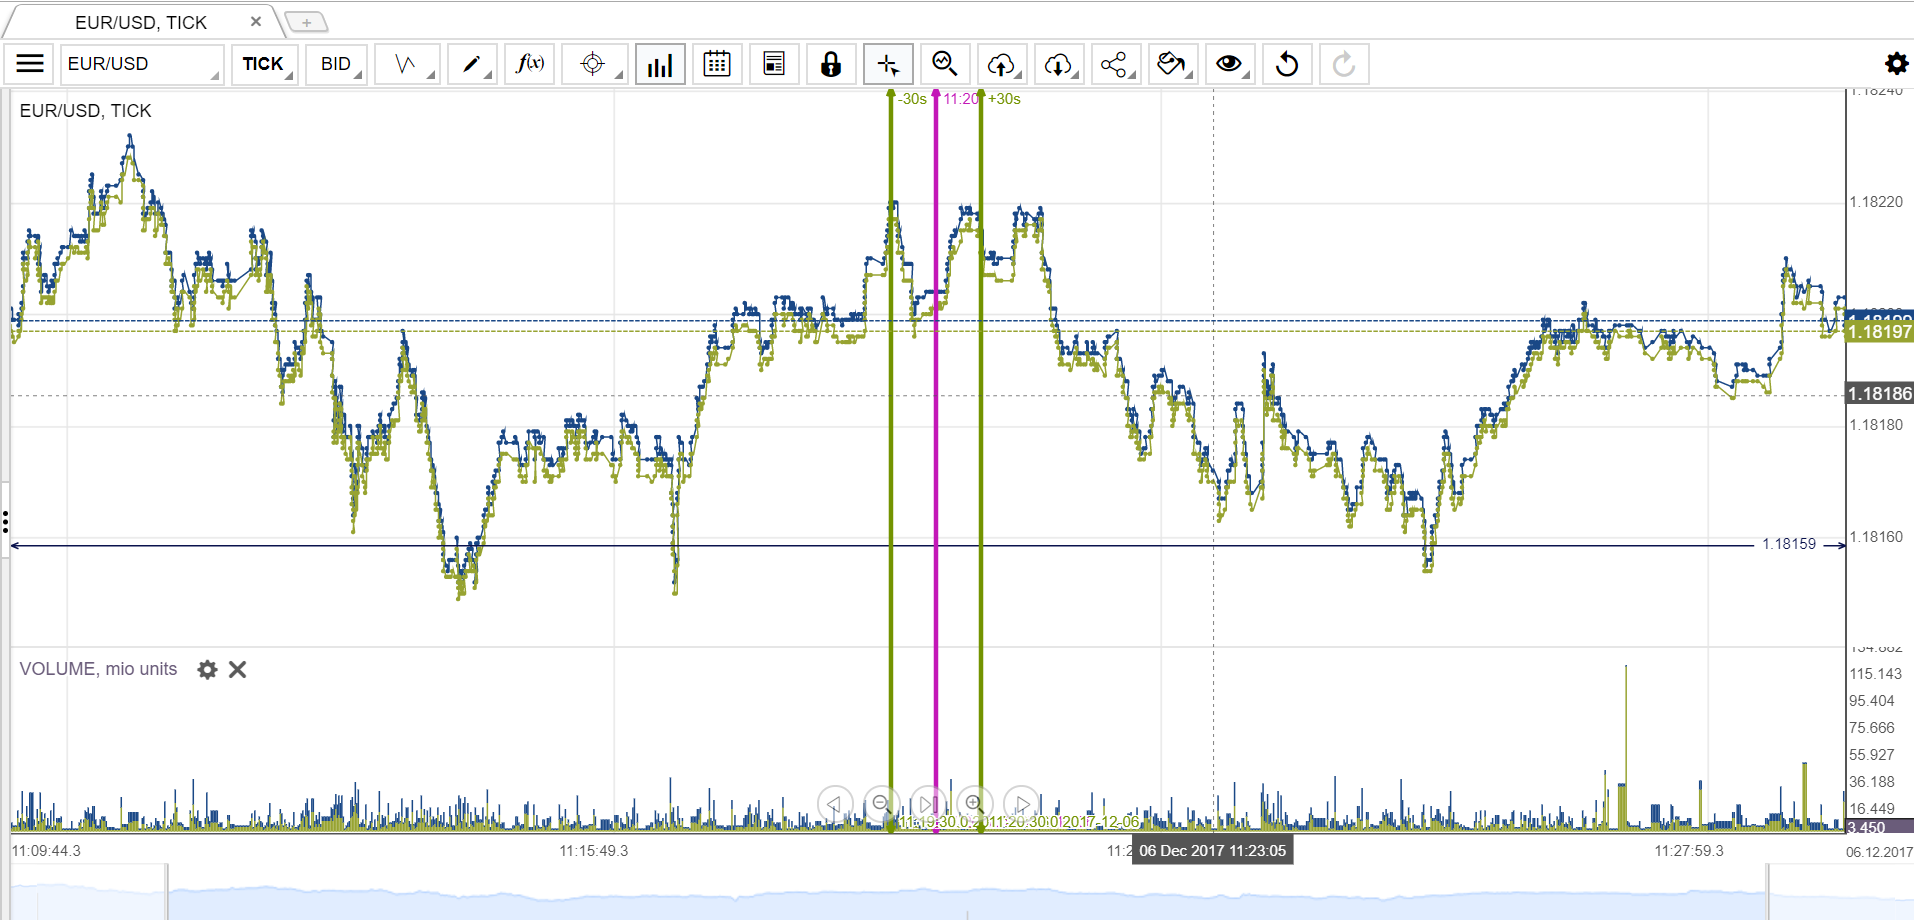
\includegraphics[width=\paperwidth]{img/hft-ticks.png}
%\end{frame}
%



%Have a slide for each of the following
%9 Problem statement or Hypothesis
%9 “Why is this a Hard Problem?”
%9 Approach or Methodology
%9 “Why is this Innovative?”
%9 Assumptions and Constraints
%9 Initial Results (Promise of Great Things to Come)
%9 Validation Plan
%9 Limitations and Applicability
%9 Expected Contributions
%9 “What’s beyond this thesis?”
%9 Roadmap of Thesis

\appendix

\begin{frame}
\frametitle{VECM(p) matrix form}
If we have $N$ data points, with $N>p$, we can estimate the model parameters $\mathbf{X}$ using the following matrix form:
\small
\begin{equation*}
\underbrace{
      \begin{bmatrix}
       \mathbf{\Delta y}_{p+1}  \\ 
       \mathbf{\Delta y}_{p+2}  \\ 
       \vdots                   \\ 
       \mathbf{\Delta y}_N      
      \end{bmatrix}}_{\mathbf{B} } =
\arraycolsep=1.4pt  
\underbrace{\begin{bmatrix}
   \alpha^\top & \phi^*_1 & \dots & \phi^*_{p-1} &\mathbf{c}   
  \end{bmatrix}}_{\mathbf{X}^\top}
\underbrace{\begin{bmatrix}
 \beta\mathbf{y}_p      & \beta\mathbf{y}_{p+1}   & \dots&   \beta\mathbf{y}_{N-1}   \\
 \mathbf{\Delta y}_{p}   & \mathbf{\Delta y}_{p+1}& \dots &  \mathbf{\Delta y}_{N-1} \\
 \mathbf{\Delta y}_{p-1} & \mathbf{\Delta y}_{p}  & \dots &  \mathbf{\Delta y}_{N-2}   \\
 \vdots                  & \vdots                 & \ddots&  \vdots                   \\
 \mathbf{\Delta y}_{2}   & \mathbf{\Delta y}_{3} & \dots &   \mathbf{\Delta y}_{N-p+1} \\
 1                      & 1                       & \dots     & 1   
 \end{bmatrix}}_{\mathbf{A}^\top}
+
\underbrace{\begin{bmatrix}
              \mathbf{\epsilon}_{p+1} \\ 
              \mathbf{\epsilon}_{p+2} \\ 
              \vdots \\ 
              \mathbf{\epsilon}_N
             \end{bmatrix}}_{\mathbf{E}^\top}
\end{equation*}
\end{frame}



\begin{frame}
\frametitle{Integration example}
\begin{columns}
\column[t]{5cm}
High frequency financial time series are commonly an I(1) process 
\begin{center}
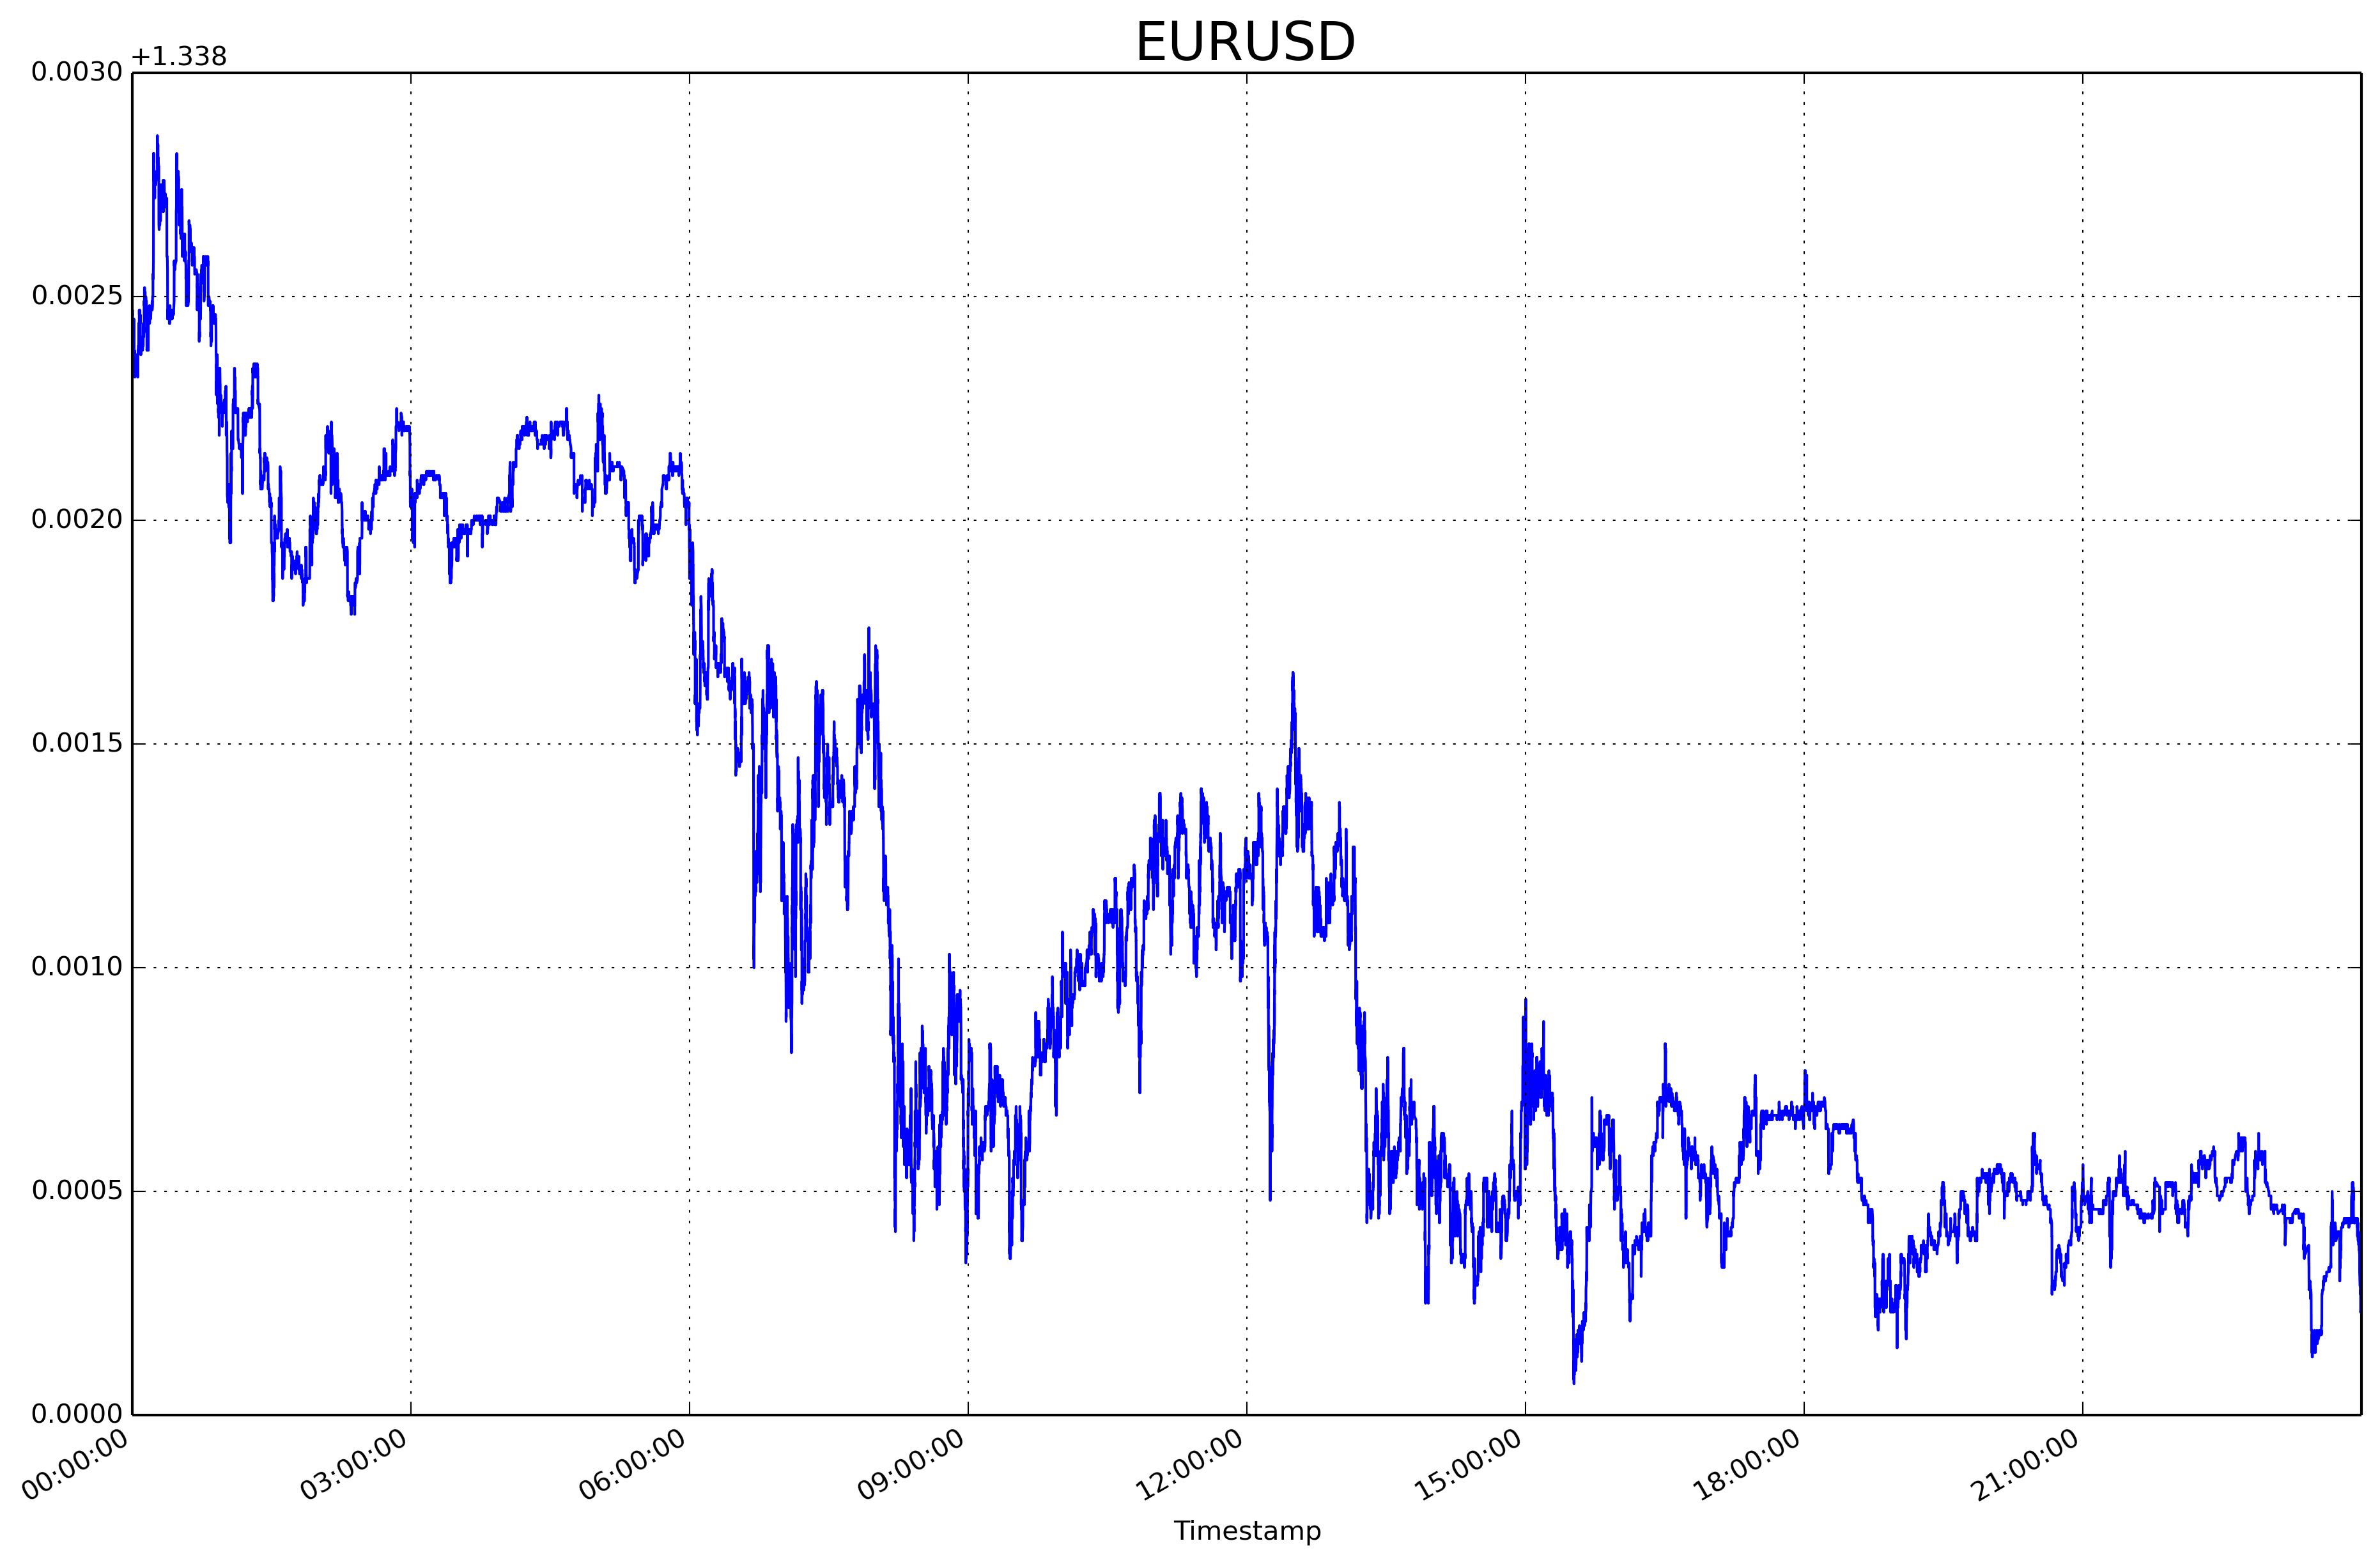
\includegraphics[width=0.85\textwidth]{img/EURUSD}
\end{center}
\column[t]{5cm}
Since their differences are stationary (I(0) process).
\newline
\begin{center}
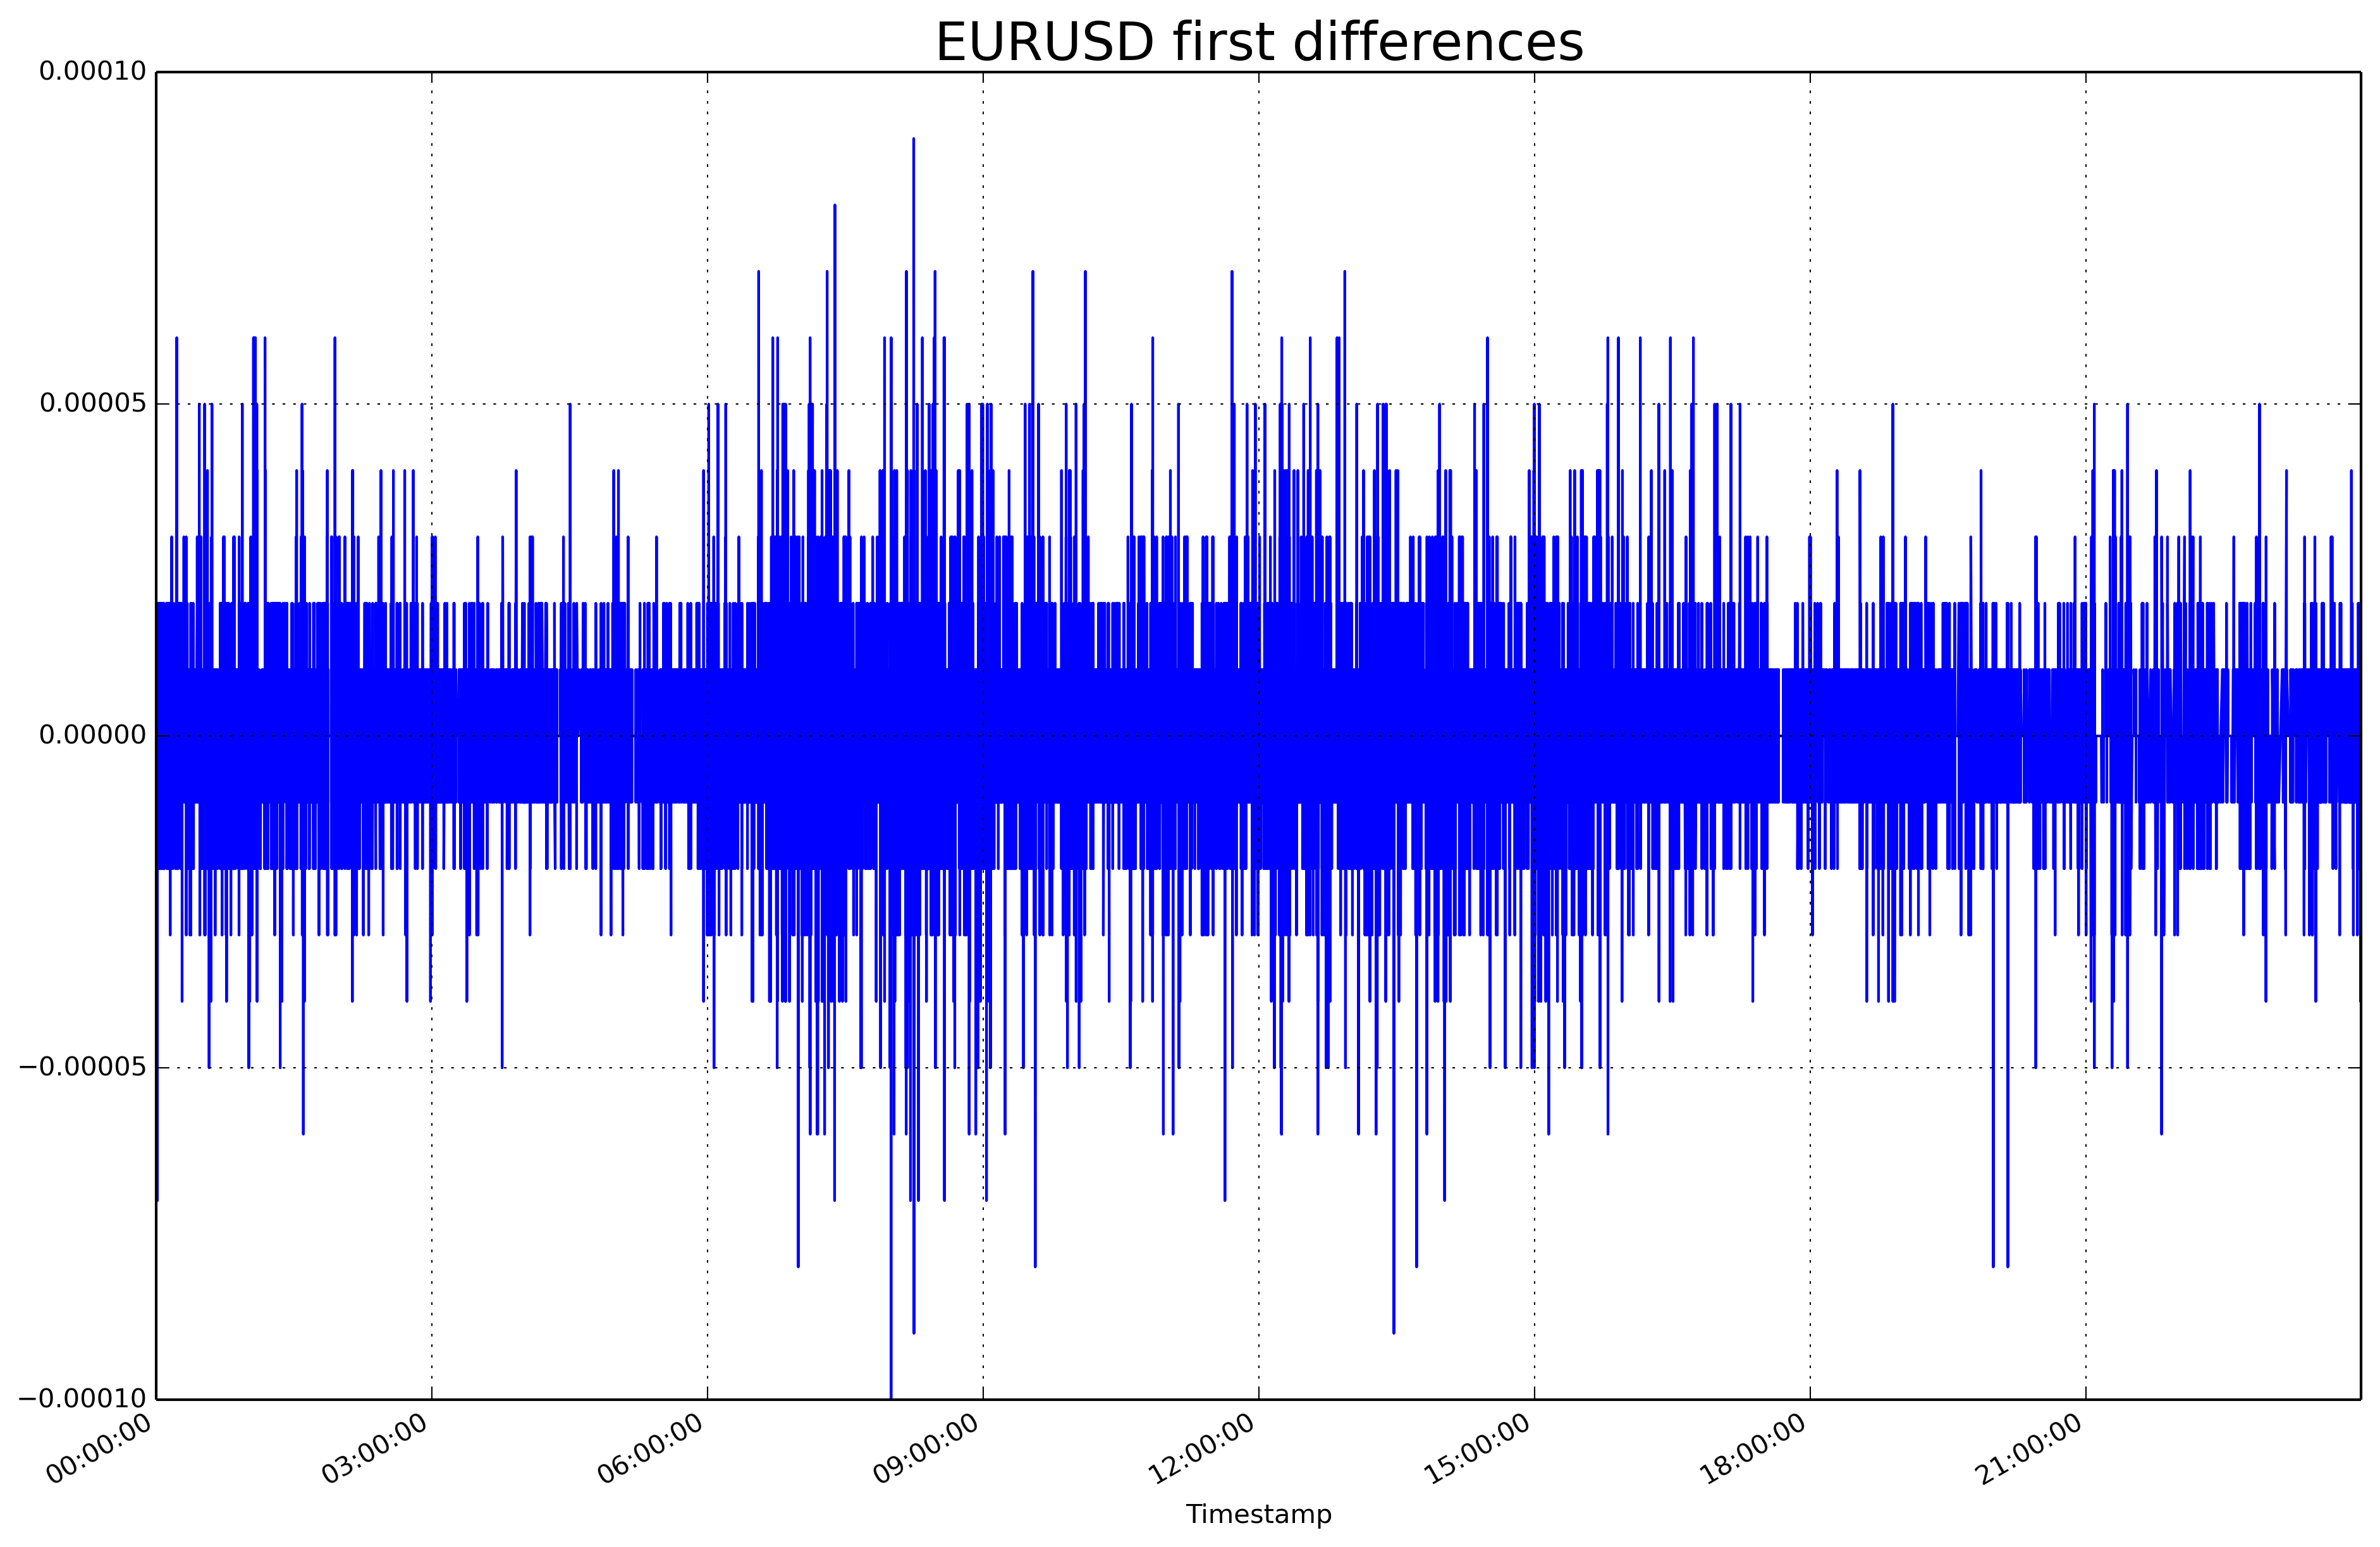
\includegraphics[width=0.85\textwidth]{img/DEURUSD}
\end{center}
\end{columns}
\end{frame}

\begin{frame}
\frametitle{Spurious regression}
Standard regression techniques are applied to non-stationary data.
The use of non-stationary data can lead to spurious regressions.  

%\begin{block}{Spurious regression}
%If two stationary
%variables are generated as independent random series and are trending over time, when one of those variables is regressed on the other, they could have a high coefficient of determination ($R^2$) even if the two are totally unrelated. 
%\end{block}

\begin{columns}
\begin{column}{.45\linewidth}<1->
\begin{figure}
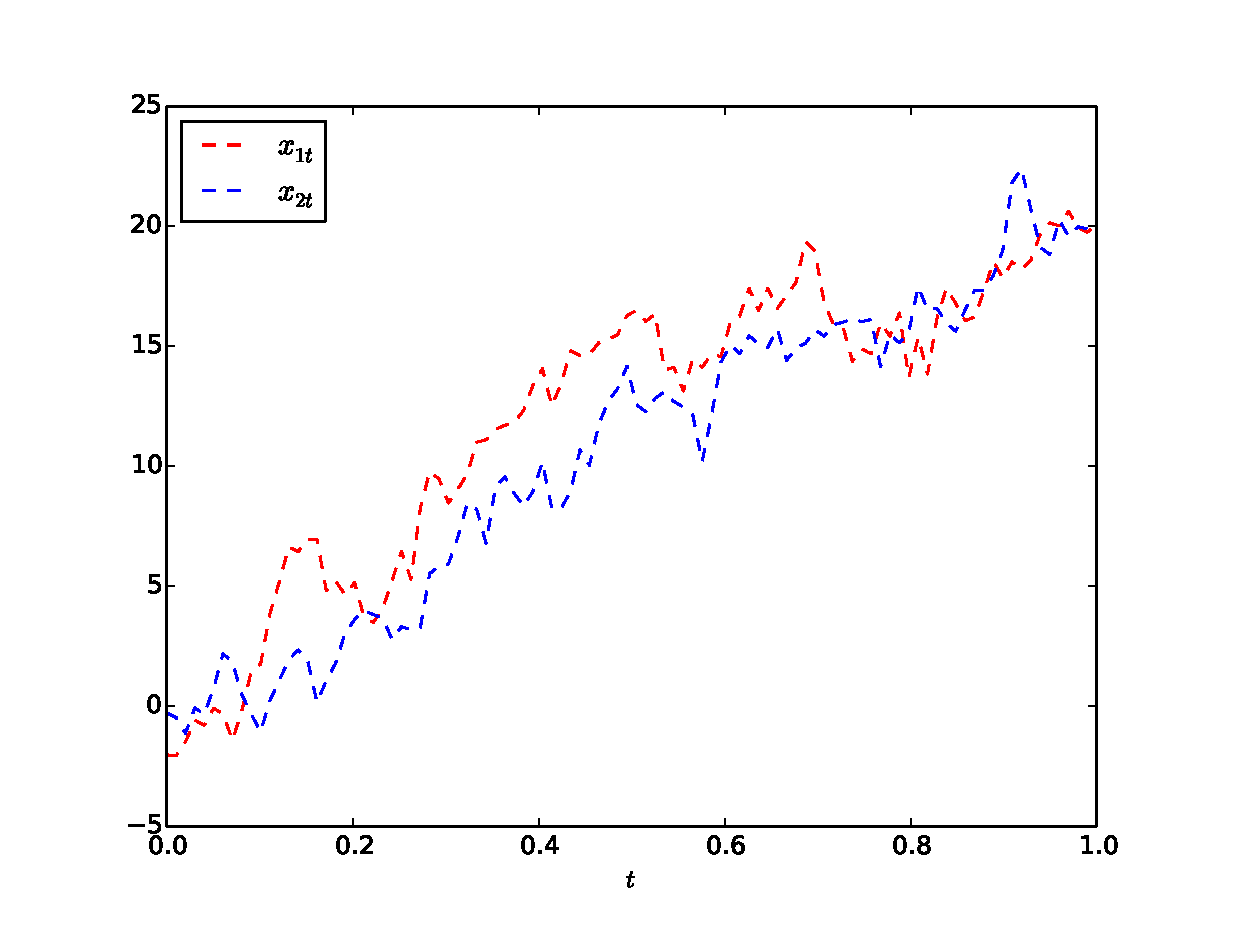
\includegraphics[width=0.4\paperwidth]{img/spurious1}
\end{figure}
\end{column}
\begin{column}{.45\linewidth}<2->
\begin{figure}
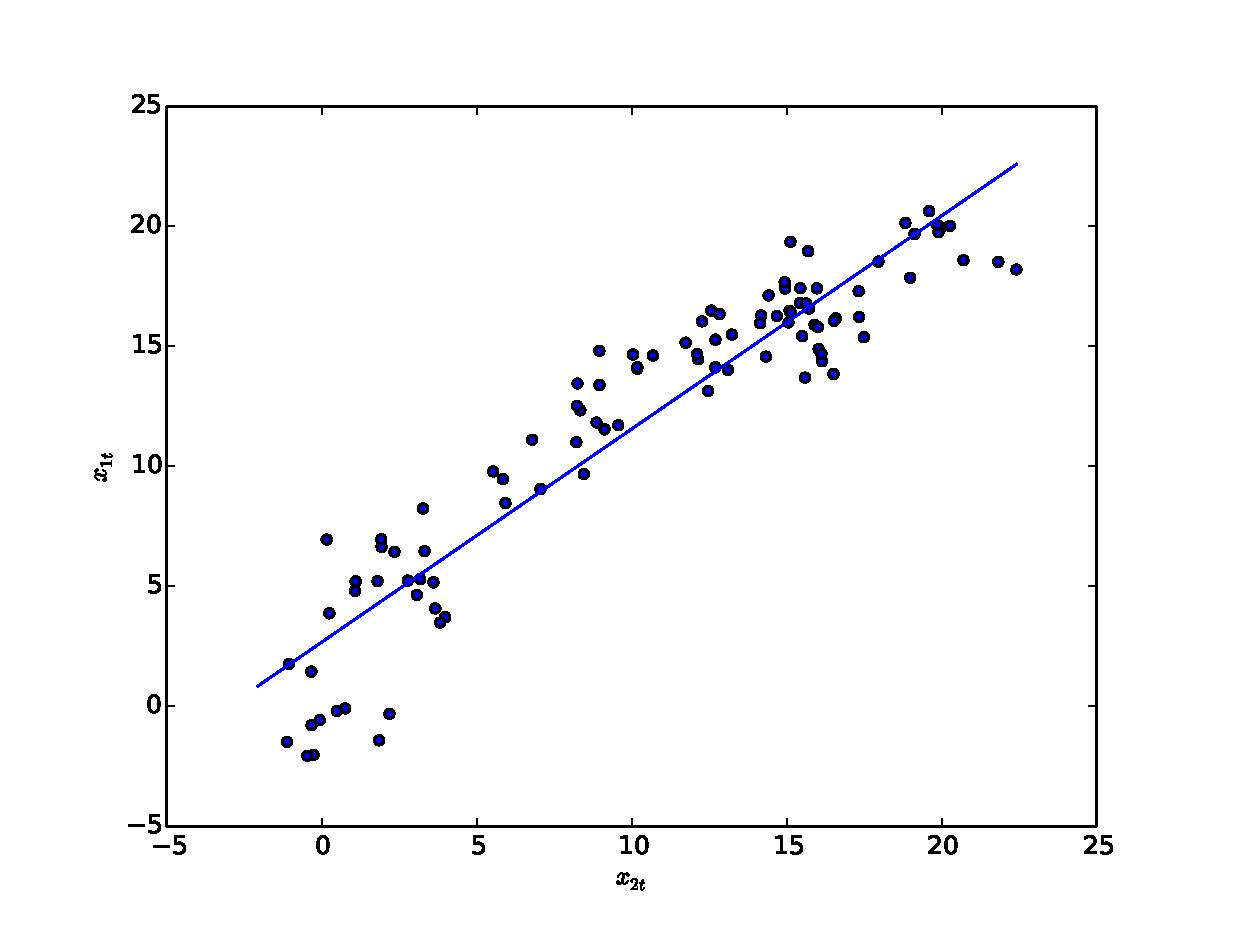
\includegraphics[width=0.4\paperwidth]{img/spurious2}
\end{figure}
\end{column}
\end{columns}
\end{frame}

%\subsection{Model comparison} 
\begin{frame}
\frametitle{Random walk}
The random walk model is defined as:
\begin{equation}
\mathbf{y}_t = \mathbf{y}_{t-1} + \epsilon_{t}
\label{rwmodel}
\end{equation}
The naive forecast of the time series difference $\hat{\mathbf{y}}_{t+1}$ for the random walk model is defined as:
\begin{equation}
\hat{\mathbf{y}}_{t+1} = \mathbf{y}_t + \hat{\epsilon}_{t+1} 
\end{equation}
\noindent where  $\hat{\epsilon}_{t+1} = \epsilon_{t}$.
\end{frame}
%
%
\begin{frame}
\frametitle{ARIMA}
A process can be modelled as an ARIMA$(p,d,q)$ if $\mathbf{x}_t = \Delta^d \mathbf{y}_t $, is an ARMA$(p,q)$. An ARMA$(p,q)$ model is the following:
\begin{equation}
\mathbf{x}_t = \sum_{i=1}^p \phi_i \mathbf{x}_{t-i}  +  \sum_{j=1}^q \theta_j \epsilon_{t-j}  
\end{equation}
\noindent with coefficients $\phi_p \neq 0$, $\theta_q \neq 0$ and $\sigma_{\epsilon}^2 > 0$.
\end{frame}


% Financial time series are not the only ones with this behaviour, this study can be extended to other non-stationary time series such as: weather, earthquakes, energy demand and sales forecasting.


\end{document}
